\subsection{Writes-follow-reads Consistency}\label{wfr:writes-follow-reads-consistency}

\subsubsection{Definition}\label{wfr:definition}

Writes-follow-reads (WFR) consistency requires a write that follows a read by the same client to be performed on the same or a more recent version than the one previously read. For example, if a client reads version 2 and then submits an update based on it, the system should preserve the dependency between the observed version and the subsequent write.

Our experiment examines an observable consequence of this dependency: whether a read-dependent update survives Cassandra's timestamp-based reconciliation. As in the MW experiment, the final winning value is an operational indicator, not a direct observation of the order in which every replica applies mutations.

\subsubsection{Experimental Design}\label{wfr:experimental-design}

Each iteration uses a fresh key. A setup write $W_a$ first stores $x=1$, followed by a preceding write $W_b$ that stores $x=2$. The client then reads the key and issues a dependent write $x=r+10$, where $r$ is the observed value. A final verification read identifies the winning version. The coordinator paths and setup and verification consistency levels vary with the topology, as specified in Table~\ref{tab:wfr-topology}.

If the client reads $r=2$, it has observed $W_b$, and the dependent write stores $x=12$. This establishes the dependency tested by the experiment. A final value of 12 indicates that the dependent update was preserved; a final value of 2 indicates that the preceding write remained the winner despite the later dependent update. If the client reads $r=1$, the trial is recorded as a stale read and excluded from the violation rate for the dependency on $W_b$.

Two modes are used. In natural mode, writes use ordinary driver-generated timestamps, and $W_b$ uses the selected write CL. In skew mode, $W_b$ receives a future-dated timestamp and uses the verification CL listed in Table~\ref{tab:wfr-topology}, establishing its visibility within the participating component before the trigger read. In both modes, the trigger read uses the selected read CL, while the dependent write uses the selected write CL and a driver-generated timestamp. The original scenario matrix used a five-second timestamp offset and recorded whether it was sufficient to produce the intended inversion. Thus, the modes differ in both timestamp assignment and the CL used for $W_b$; their trigger rates should not be interpreted as a comparison that changes timestamps alone.

The scenario matrix contains 64 configurations: two delay/jitter settings, four operational scenarios, four write/read CL combinations, and two modes. Each configuration has 100 attempted iterations. The operational scenarios are normal operation, single-node failure, majority partition, and minority partition; the network settings are 0/0 ms and 100/50 ms delay/jitter.

\begin{table}[H]
\centering
\small
\renewcommand{\arraystretch}{1.15}
\caption{WFR setup and verification configurations by topology. In the coordinator path, node numbers denote cass1, cass2, and cass3; the order is $W_a/W_b$, trigger read, dependent write, and verification read.}
\label{tab:wfr-topology}
\begin{tabular}{@{}
>{\RaggedRight\arraybackslash}p{(\linewidth - 8\tabcolsep) * \real{0.24}}
>{\RaggedRight\arraybackslash}p{(\linewidth - 8\tabcolsep) * \real{0.14}}
>{\RaggedRight\arraybackslash}p{(\linewidth - 8\tabcolsep) * \real{0.17}}
>{\RaggedRight\arraybackslash}p{(\linewidth - 8\tabcolsep) * \real{0.29}}
>{\RaggedRight\arraybackslash}p{(\linewidth - 8\tabcolsep) * \real{0.16}}@{}}
\toprule
Scenario & Setup CL & Verification CL & Coordinator path & Settle time (ms) \\
\midrule
Normal & ALL & ALL & $1\to2\to3\to1$ & 0 \\
Node failure & QUORUM & QUORUM & $1\to2\to1\to1$ & 1000 \\
Majority partition & QUORUM & QUORUM & $1\to2\to1\to1$ & 1000 \\
Minority partition & ONE & ONE & $3\to3\to3\to3$ & 1000 \\
\bottomrule
\end{tabular}
\end{table}

No additional client-side sleep is inserted between $W_b$ and the trigger read. The settling interval in Table~\ref{tab:wfr-topology} occurs only after the dependent write and before verification. Verification covers all three replicas in the normal topology, the two reachable replicas under node failure or majority partition, and only cass3 in the minority partition. The fixed settling interval is not itself proof of convergence, and partition-local verification does not establish convergence across the partition.

The additional delay plots present natural and skew results at 0, 5, 10, 20, and 50 ms with zero configured jitter. These scanning results are discussed separately from the scenario matrix.

\begin{figure}[H]
\centering
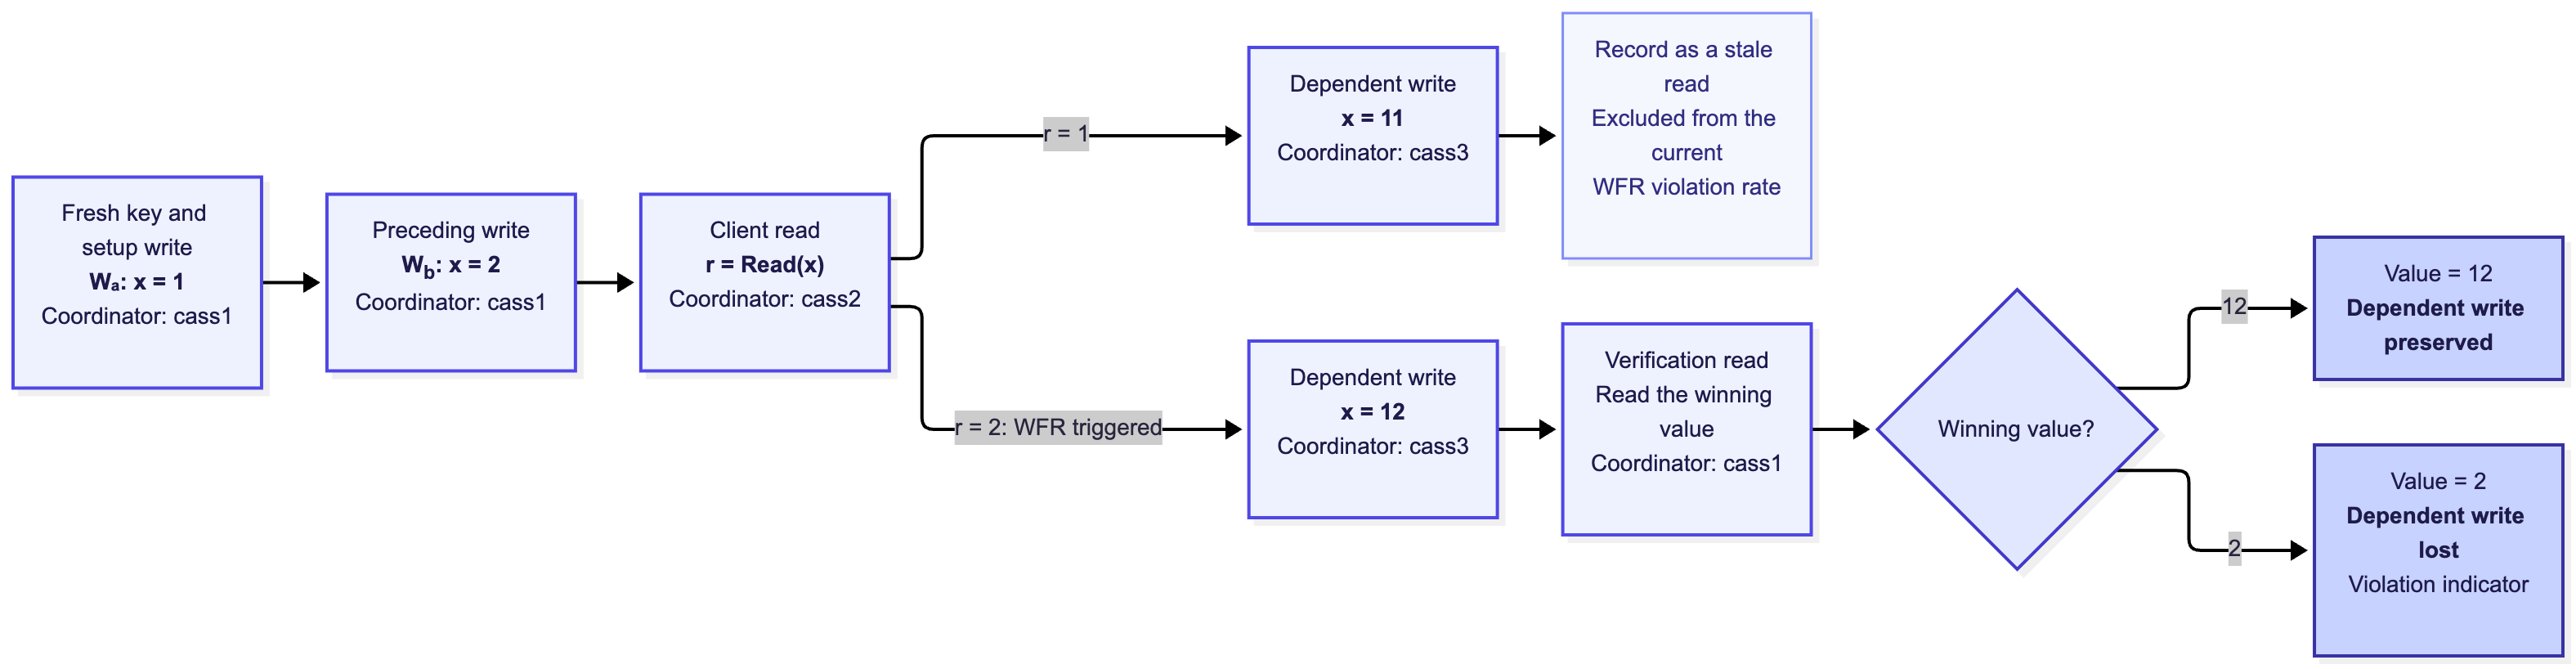
\includegraphics[width=\linewidth]{figures/wfr_flow.png}
\caption{Writes-follow-reads experimental workflow under the normal topology.}
\label{fig:wfr-flow}
\end{figure}

\subsubsection{Principle and Key Implementation}\label{wfr:principle-and-key-implementation}

The analysis distinguishes three outcomes: operation completion, visibility of the preceding write, and preservation of the dependent update.

Operation errors, including unavailable and timeout outcomes, are recorded separately from consistency violations. Among completed trials, the trigger rate measures how often the client reads \(x=2\). The measured WFR violation rate is:

\begin{equation}
\text{Violation rate} =
\frac{\text{triggered trials in which the dependent update is lost}}
{\text{triggered trials}}.
\end{equation}

A configuration with no triggered trials has an undefined violation rate, not a measured rate of 0\%. Such points must therefore appear as gaps in the plots.

For the preceding write and trigger read in natural mode, with RF=3, QUORUM/QUORUM and ALL/ONE satisfy \(R+W>N\), whereas ONE/ONE and ONE/QUORUM do not. Replica overlap helps explain whether the client observes \(W_b\), but it does not determine the ordering of timestamps assigned to competing writes. Even if every replica receives the dependent update, Cassandra's last-write-wins reconciliation can retain \(W_b\) when its timestamp is greater.

\subsubsection{Predicted Outcomes}\label{wfr:predicted-outcomes}

In natural mode, if the dependent write receives a later timestamp than \(W_b\), it should win reconciliation after successful verification. Replication delay may reduce the probability that the preceding read observes \(W_b\), particularly under weak CL combinations, without necessarily causing the dependent update to lose once the test is triggered.

In skew mode, if the future-dated timestamp of \(W_b\) remains greater than that of the dependent write, \(x=2\) should remain the winning value. Increasing the write or read CL should not reverse this timestamp ordering.

{
\begin{table}[H]
\centering
\small
\renewcommand{\arraystretch}{1.15}
\caption{Predicted WFR outcomes conditional on successful operations and a triggered check.}\label{tab:wfr-1}
\begin{tabular}{@{}
  >{\RaggedRight\arraybackslash}p{(\linewidth - 6\tabcolsep) * \real{0.2500}}
  >{\RaggedRight\arraybackslash}p{(\linewidth - 6\tabcolsep) * \real{0.2500}}
  >{\RaggedRight\arraybackslash}p{(\linewidth - 6\tabcolsep) * \real{0.2500}}
  >{\RaggedRight\arraybackslash}p{(\linewidth - 6\tabcolsep) * \real{0.2500}}@{}}
\toprule\noalign{}
\begin{minipage}[b]{\linewidth}\RaggedRight
Timestamp mode
\end{minipage} & \begin{minipage}[b]{\linewidth}\RaggedRight
Condition
\end{minipage} & \begin{minipage}[b]{\linewidth}\RaggedRight
Expected winning value in triggered trials
\end{minipage} & \begin{minipage}[b]{\linewidth}\RaggedRight
Expected measured violation rate
\end{minipage} \\
\midrule\noalign{}
Natural & Dependent write has the later timestamp & 12 & 0\% \\
Skew & \(W_b\) retains the greater timestamp & 2 & 100\% \\
\bottomrule
\end{tabular}
\end{table}
}

These predictions are conditional on successful operations and a triggered check. Failures and partitions are expected to make configurations requiring unreachable replicas unavailable, rather than produce valid consistency observations.

\subsubsection{Results and Analysis}\label{wfr:actual-results-and-analysis}

\paragraph{Delay-scan Results}\label{wfr:delay-scan-results}

\begin{figure}[htbp]
\centering
\begin{subfigure}{\linewidth}
\centering
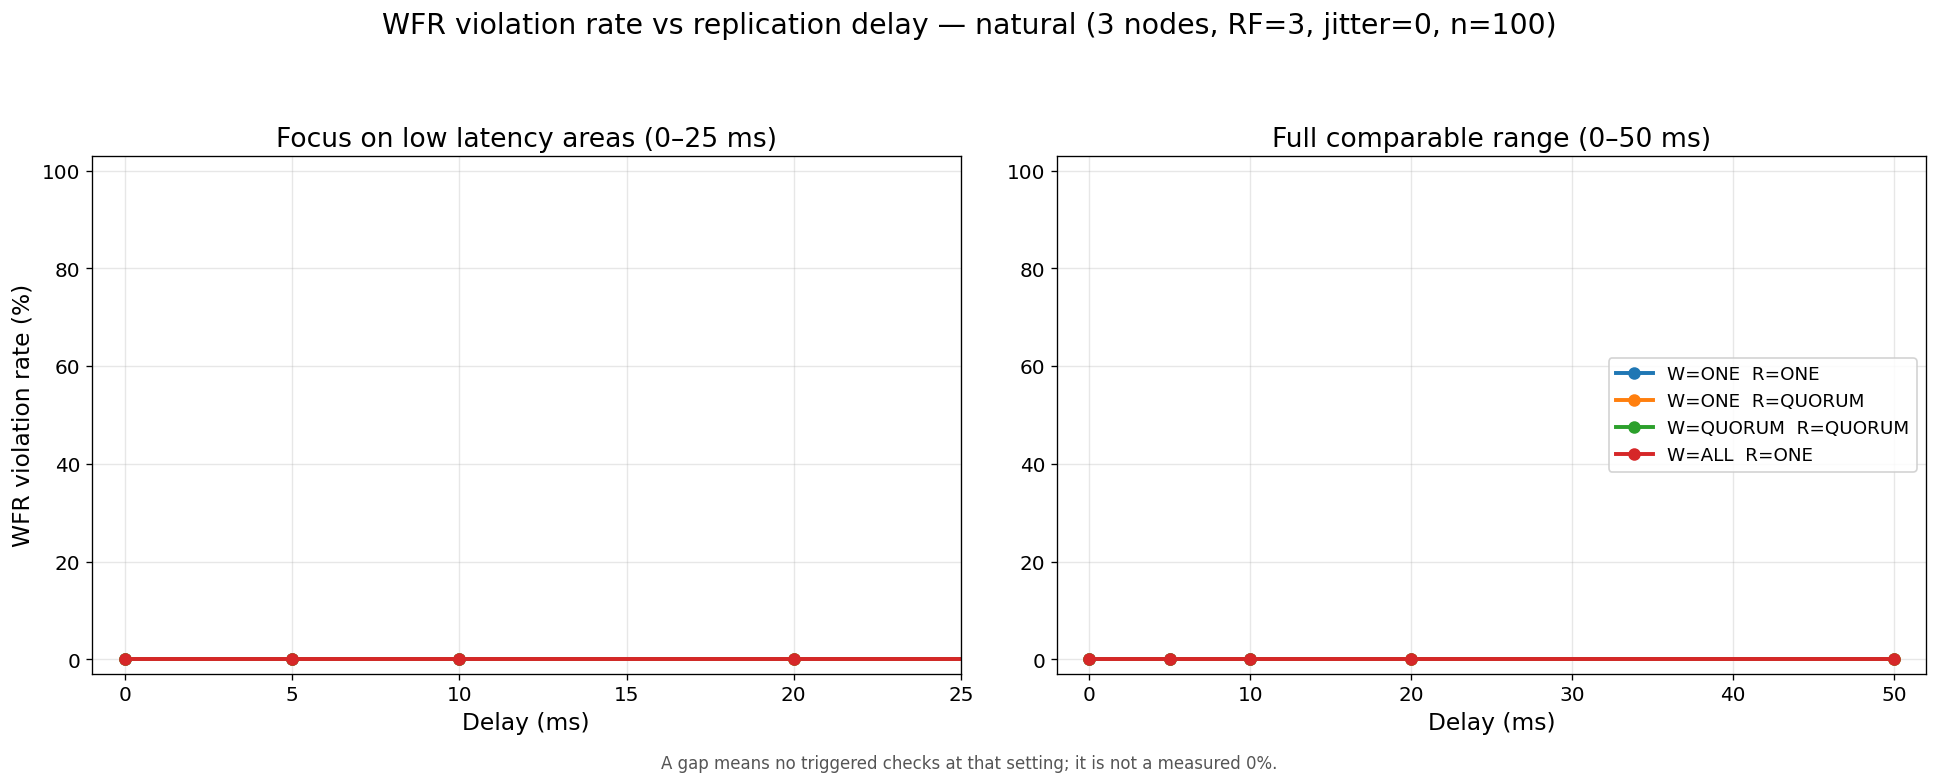
\includegraphics[width=\linewidth]{figures/wfr_natural.png}
\caption{Natural mode}
\end{subfigure}
\par\medskip
\begin{subfigure}{\linewidth}
\centering
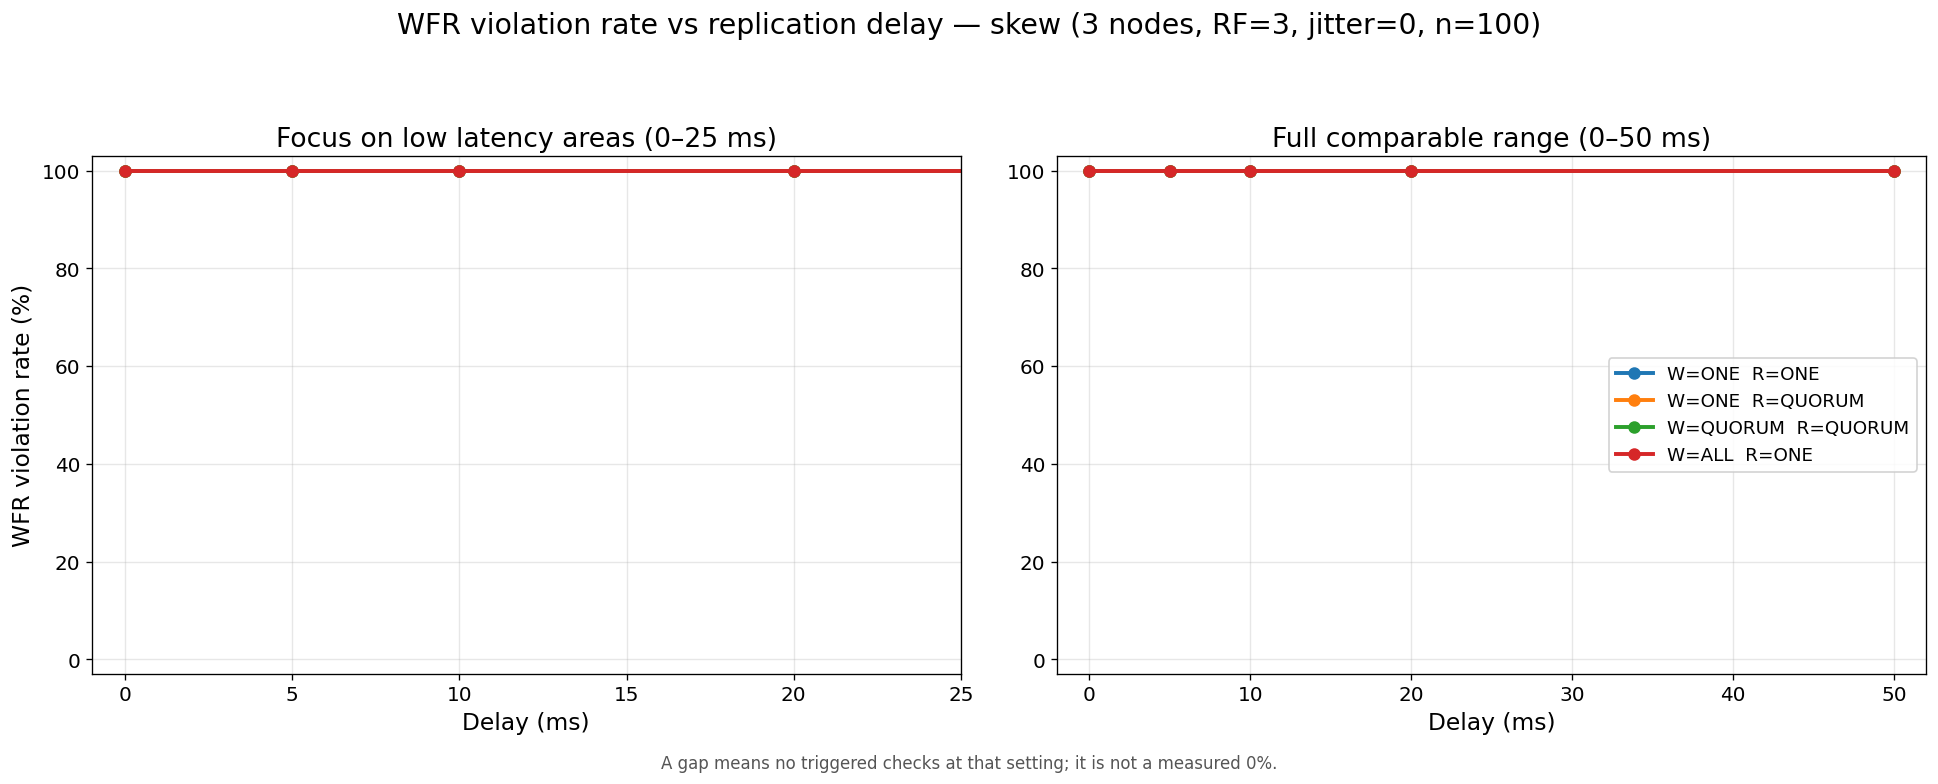
\includegraphics[width=\linewidth]{figures/wfr_skew.png}
\caption{Skew mode}
\end{subfigure}
\par\medskip
\caption{WFR violation rate versus injected replication delay, with RF=3 and jitter=0. Each mode includes a low-delay view and a full displayed range of 0--50 ms. The plots report $n=100$ iterations per configuration; the violation-rate denominator is the number of triggered checks. Gaps indicate settings without triggered checks.}
\label{fig:wfr-delay}
\end{figure}

The delay plots show a clear separation between timestamp modes. In natural mode, all displayed valid observations have a measured violation rate of 0\%. In skew mode, all displayed valid observations have a rate of 100\%. Curves with identical values overlap, so the visible red line should not be interpreted as representing only ALL/ONE. Conversely, an overlapping curve can conceal a gap in another series; a visible line does not establish that every configuration has valid observations at every delay.

Unlike the RYW and MR experiments, the displayed WFR results do not show an increasing violation rate as replication delay grows. This difference follows from the measured event. RYW and MR expose cases in which reads observe missing or older versions during delayed propagation. The WFR indicator is evaluated only after the client has observed \(W_b\), and then checks whether the dependent update survives reconciliation.

In natural mode, the zero-rate observations are consistent with the dependent update receiving a later timestamp and remaining the winner. They do not show that every preceding read was fresh, or that every attempted iteration triggered a WFR check. Replication delay can affect those quantities without changing the conditional violation rate.

The skew-mode results show the opposite outcome. The dependent update loses even under QUORUM/QUORUM and ALL/ONE. Stronger replica acknowledgements therefore do not correct the deliberately inverted timestamp order. This agrees with the MW findings: application order and timestamp order are different, and increasing consistency levels does not make reconciliation follow application order when the supplied timestamps conflict with it.

\FloatBarrier
\paragraph{Results Across Operational Scenarios}\label{wfr:results-across-operational-scenarios}

The original scenario matrix provides complementary evidence about visibility and availability.

{
\begin{table}[H]
\centering
\small
\renewcommand{\arraystretch}{1.15}
\caption{WFR results in the original 64-configuration scenario matrix, excluding the additional delay scan.}\label{tab:wfr-2}
\begin{tabular}{@{}
  >{\RaggedRight\arraybackslash}p{(\linewidth - 10\tabcolsep) * \real{0.1304}}
  >{\raggedleft\arraybackslash}p{(\linewidth - 10\tabcolsep) * \real{0.1739}}
  >{\raggedleft\arraybackslash}p{(\linewidth - 10\tabcolsep) * \real{0.1739}}
  >{\raggedleft\arraybackslash}p{(\linewidth - 10\tabcolsep) * \real{0.1739}}
  >{\raggedleft\arraybackslash}p{(\linewidth - 10\tabcolsep) * \real{0.1739}}
  >{\raggedleft\arraybackslash}p{(\linewidth - 10\tabcolsep) * \real{0.1739}}@{}}
\toprule\noalign{}
\begin{minipage}[b]{\linewidth}\RaggedRight
Mode
\end{minipage} & \begin{minipage}[b]{\linewidth}\raggedleft
Attempted iterations
\end{minipage} & \begin{minipage}[b]{\linewidth}\raggedleft
Completed iterations
\end{minipage} & \begin{minipage}[b]{\linewidth}\raggedleft
Triggered checks
\end{minipage} & \begin{minipage}[b]{\linewidth}\raggedleft
Measured violations
\end{minipage} & \begin{minipage}[b]{\linewidth}\raggedleft
Unavailable or timeout outcomes
\end{minipage} \\
\midrule\noalign{}
Natural & 3,200 & 2,200 & 1,896 & 0 & 1,000 \\
Skew & 3,200 & 2,200 & 2,200 & 2,200 & 1,000 \\
\bottomrule
\end{tabular}
\end{table}
}

These totals refer only to the original 64-configuration matrix, not the additional delay scan.

In natural mode, the 304 completed but untriggered iterations returned the stale value \(r=1\). At zero injected delay, every available configuration achieved a 100\% trigger rate. With 100 ms delay and 50 ms jitter, the normal-topology trigger rate fell to 8\% for ONE/ONE and 79\% for ONE/QUORUM, while QUORUM/QUORUM and ALL/ONE retained 100\%. ONE/ONE also produced low trigger rates under single-node failure and majority partition: 3\% and 6\%, respectively.

These differences are consistent with the replica-overlap argument used in the preceding experiments. ONE/QUORUM can improve visibility relative to ONE/ONE, but \(R+W=N\) does not guarantee overlap. The stronger combinations satisfy \(R+W>N\), consistent with their observed visibility when operations complete. Nevertheless, none of the 1,896 triggered natural-mode checks detected loss of the dependent update.

In skew mode, all 2,200 completed iterations triggered the check and ended with the dependent update losing. The recorded timing checks reported no completed iteration in which the configured skew was too small. The results therefore support the intended timestamp-inversion explanation for this matrix.

Failures and partitions also restricted operation completion. ALL/ONE could not complete after a node failure or within either partition component because all three replicas were not reachable. On the isolated minority, only ONE/ONE completed the WFR sequence. These unavailable outcomes provide availability evidence and must not be interpreted as zero-violation results.

\paragraph{Interpretation and Limitations}\label{wfr:interpretation-and-limitations}

Taken together, the experiments separate visibility, availability, and timestamp ordering. Consistency levels and replication delay affected whether the client observed the preceding write, while network reachability affected whether the sequence could complete. Conditional on a triggered and successfully verified check, the timestamp modes produced opposite outcomes: the dependent update survived in natural mode and lost under the tested timestamp inversion.

The scope of this conclusion is limited by the measurement. The experiment observes the final reconciled value rather than each replica's causal history, and deliberately assigned timestamps do not reproduce all effects of independent machine-clock drift. The displayed scan also covers a finite set of delays and iterations. The results therefore characterize the tested read-dependent-update workload, rather than constitute a complete formal verification of WFR.
